% \documentclass{beamer} %First Page Setup
% \usetheme{Singapore}%{Warsaw} %First Page Setup
% \usetheme{Boadilla}

%=============================First Page Setup==============================================
\documentclass[xcolor=dvipsnames]{beamer}

%--
\usepackage{hyperref}
\usepackage[utf8]{inputenc} % this is needed for german umlauts
\usepackage[brazil]{babel} % this is needed for german umlauts
\usepackage[T1]{fontenc}    % this is needed for correct output 
                            % of umlauts in pdf

\usepackage{graphicx,url}
\usepackage{amsmath, amsthm, amssymb, amsfonts}
% \usepackage{amssymb}
\usepackage[binary-units]{siunitx}
\usepackage{subfigure}
\usepackage{textcomp}

\setbeamertemplate{caption}[numbered] %Figs numbered
%--

\defbeamertemplate*{title page}{customized}[1][]
{
\usebeamerfont{subtitle}
\usebeamercolor[fg]{subtitle}

{\flushright
\setbeamercolor{author}{bg=white,fg=Blue} %Red
\usebeamerfont{author} \insertauthor\par
\usebeamerfont{institute}\insertinstitute\par }

\vspace{0.2in}

\setbeamercolor{postit}{fg=white,bg=Blue} %YellowOrange

\begin{beamercolorbox}[sep=1em,wd=1.062\textwidth,ht=3cm,dp=3cm,right]{postit}
\usebeamerfont{title} {\huge \inserttitle}\par
\usebeamerfont{subtitle} {\insertsubtitle}
\end{beamercolorbox}
}
\usecolortheme[named=Blue]{structure} %YellowOrange
\useoutertheme{infolines}
\setbeamertemplate{navigation symbols}{} 
\institute{Laboratório de Computação Cienífica e Análise Numérica\\ Universidade Federal de Alagoas (LaCCAN-UFAL)}

\title{Avaliação de Geradores de Números Pseudoaleatórios Através de Técnicas da Teoria da Informação}
\subtitle{ERAD-NE 2015}
\titlegraphic{
\includegraphics[width=0.5cm]{logo-laccan}}
\author{Marcelo Q.\ A.\ Oliveira, Tamer S.\ G.\ Cavalcante, \\Heitor S.\ Ramos, Osvaldo A. Rosso, Alejandro C.\ Frery}

%=============================First Page Setup==============================================

\AtBeginSection[]
{
  \begin{frame}<beamer>
    \frametitle{Agenda} %\thesection
    \tableofcontents[currentsection]
  \end{frame}
}
                           
\begin{document}
% \title{Avaliação de Geradores de Números Pseudoaleatórios \\ Através de Técnicas da Teoria da Informação}

% \author{Marcelo Q.\ A.\ Oliveira, Tamer S.\ G.\ Cavalcante, \\Heitor S.\ Ramos, Osvaldo A. Rosso, Alejandro C.\ Frery}

% \address{Laboratório de Computação Cienífica e Análise Numérica\\ Universidade Federal de Alagoas (LaCCAN-UFAL)}

% \email{\{marceloqao,tamersgc,heitor.ramos,oarosso,acfrery\}@gmail.com}

% ---
% \author{Martin Thoma}
\date{06 de Novembro de 2015}
\subject{Computer Science}
% \frame{\titlepage}
\setbeamertemplate{footline}{} %First Page setup
\begin{frame} %First Page setup
\titlepage %First Page setup
\end{frame} %First Page setup


\section{Introdução}
\begin{frame}{Introdução}
    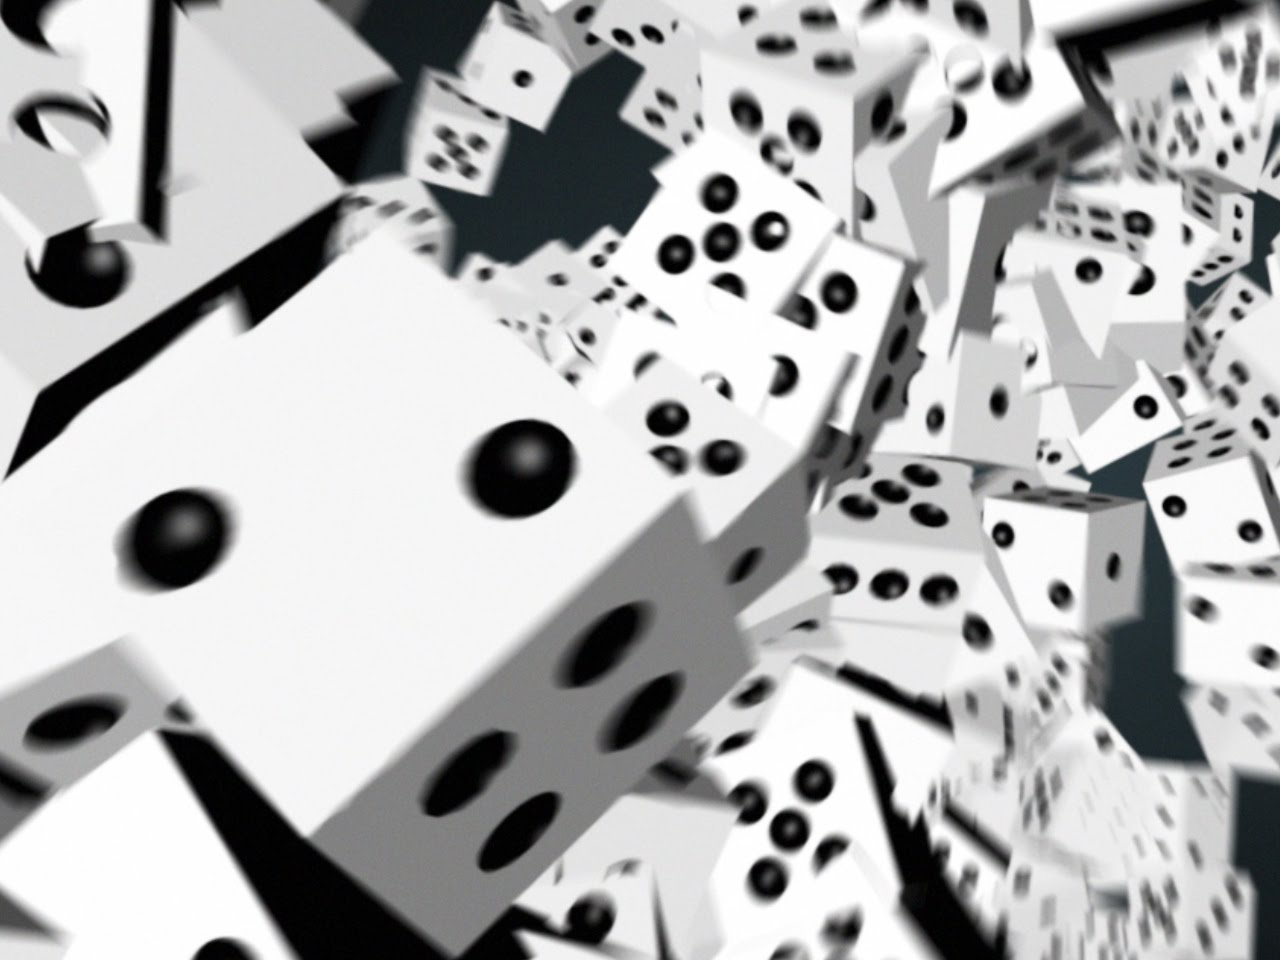
\includegraphics[width=5cm]{dices}
\end{frame}

\subsection{Motivação}
\begin{frame}{Motivação}
    \begin{itemize}
     \item Criptografia
     \pause
     \item Amostragem
     \pause
     \item Aplicações gráficas
     \pause
     \item Games
     \pause
     \item \textbf{Simulação}
    \end{itemize}
\end{frame}

\section{Números Aleatórios}
\subsection{Geradores Reais}
  \begin{frame}{Geradores Reais}
    \begin{block}{Baseados em algum fenômeno natural aleatório}
      \begin{itemize}
	\item Ruído atmosférico capturado por um rádio ~\cite[(random.org)]{RANDOM.ORG}.
	\pause
	\item Tempo entre emissão de partículas durante o decaimento radioativo ~\cite[HOTBITS]{HOTBITS}
	\pause
	\item Ruído térmico oriundo de semicondutores em um circuito (Intel Ivy Bridge)~\cite[]{IVY.REPORT} ~\cite[]{IVY.TROJAN}
	\pause
	\item Monitoramento de ruído em ambientes ~\cite{audio.entropy}.
	\pause
% 	\item Monitoramento do movimentos de lavalamps (SGI)
% 	\pause
      \end{itemize}
    \end{block}
    \begin{block}{Desvantagens}
      \begin{itemize}
	\item Necessitam de Hardware específico
	\pause
	\item Não reprodutíveis
      \end{itemize}
    \end{block}
  \end{frame}

\subsection{Geradores de Números Pseudoaleatórios}
\begin{frame}{Geradores de Números Pseudoaleatórios:}
  \begin{block}{Geradores de Números Pseudoaleatórios - PRNGs:}
    \begin{itemize}
      \item Algorítmicos (determinísticos)
      \pause
      \item Produzem sequências que se comportam como as produzidas por geradores reais a partir de sementes conhecidas~\cite{LEcuyer:98}
      \pause
      \item Mais convenientes por não necessitar de hardware específico
      \pause
      \item Possibilitam a reprodutibilidade
      \pause
    \end{itemize}
  \end{block}
\end{frame}

\begin{frame}{Período de um gerador}
    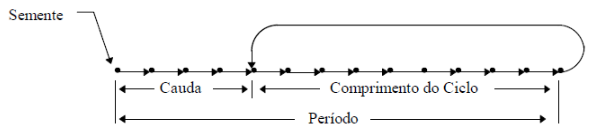
\includegraphics[width=\textwidth]{periodo}
\end{frame}

\begin{frame}{Geradores de Números Pseudoaleatórios \- PRNGs}
  \begin{block}{Propriedades desejáveis em PRNGs:}
    \begin{itemize}
      \item O período de repetição seja suficientemente grande.
      \pause
      \item A geração de números deve ser rápida.
      \pause
      \begin{itemize}
	\item Poupar recursos computacionais para as aplicações em si.
      \end{itemize}
      \pause
      \item Os números gerados devem seguir uma distribuição uniforme.
      \pause
      \begin{itemize}
	\item Devem ter a mesma probabilidade de ocorrência.
      \end{itemize}
      \pause
      \item Os números devem ser estatisticamente independentes entre si.
      \pause
      \begin{itemize}
	\item O valor de um número na sequência não deve afetar o valor do próximo.
      \end{itemize}
      \pause
    \end{itemize}
  \end{block}
\end{frame}

\begin{frame}{Método Congruencial Linear (LCG)}
Sejam os números uniformes inteiros $U1, U2, U3,$ \dots  entre $0$ e $m$ - $1$, em que $m$ representa um grande número inteiro.
Podemos gerar estes números utilizando o método congruencial por meio da relação recursiva:
 \pause
 \begin{block}{LCG}
  \begin{equation*}
    U_i+1 = (aU_i + c) mod \ m
  \end{equation*}
 \end{block}
 \pause
 \begin{block}{Onde:}
  \begin{itemize}
   \item $m$ é chamado de módulo;
   \item $a$ e $c$, inteiros positivos denominados multiplicador e incremento respectivamente;
   \item $mod$ é um operador que retorna o resto da divisão de $a_Ui + c$ por $m$;
  \end{itemize}
 \end{block}
\end{frame}

\begin{frame}{Mersenne Twister - MT}
  \begin{block}{Mersenne Twister - Matsumoto \cite{Matsumoto:MT}}
    \begin{itemize}
      \item Entrega inteiros de $32$ bits.
      \pause
      \item Período de $2^{19937}$-$1$.
      \pause
      \item Passa na maioria dos testes conhecidos.
      \end{itemize}
  \end{block}
\end{frame}


\section{Testes}
\begin{frame}{Suítes}
  \begin{itemize}
   \item Diehard (FORTRAN) \cite{Marsaglia:14}
   \pause
   \item NIST \cite{NIST:99}
   \pause
   \item Dieharder (ANSI C) \cite{Brown:04}
   \pause
   \item TEST U01 (biblioteca em ANSI C) \cite{LEcuyer:07}
  \end{itemize}

\end{frame}

\section{Ferramentas da Teoria da Informação}
\begin{frame}{Plano Entropia x Complexidade}
      \begin{figure}
      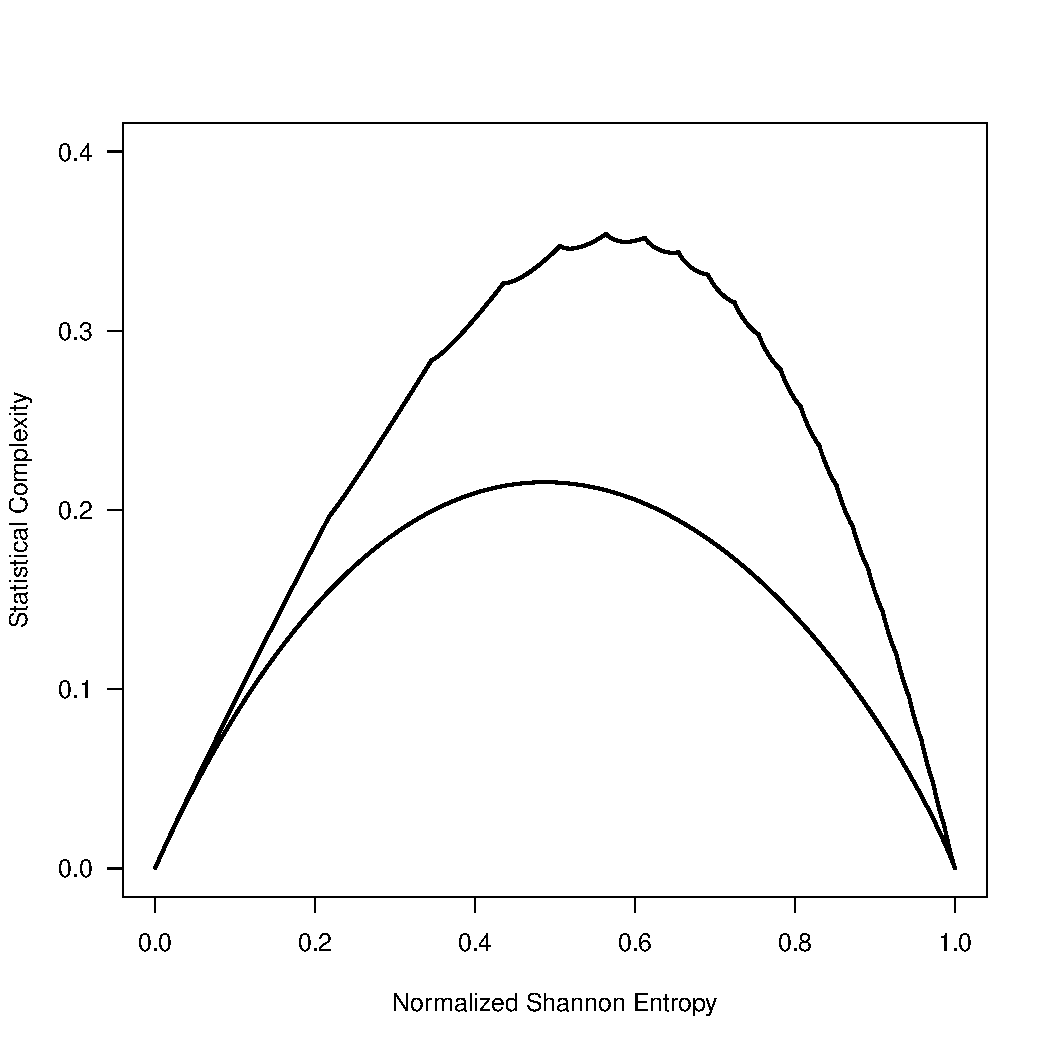
\includegraphics[scale=0.4,center]{plano-HC}
      \caption{Plano HC - Entropia x Complexidade Estatística}
      \end{figure}
\end{frame}

\section{Teste Proposto}
\begin{frame}{Teste Proposto}
    \begin{itemize}
     \item Teste de hipóteses não paramétrico para medir a qualidade da sequência gerada por um PRNG através da posição do ponto observado no plano (HC).
     \pause
     \item Com o objetivo de ter uma referência foram utilizados dados oriundos de um gerador real.
     \pause
     \item Os dados foram fornecidos pelo grupo de Processamento de Informação Quântica do Instituto de Tecnologia Max Plank, num arquivo binário  de aproximadamente 200Mb obtido segundo o processo descrito em~\cite{Gabriel2010}.
    \end{itemize}
\end{frame}

\begin{frame}{Teste Proposto}
    \begin{itemize}
     \item Tais dados foram mapeados como uma sequência de 108 números aleatórios no intervalo $(0,1)$, e então particionados em $10^5$ sequências de $10^3$ elementos cada uma.
     \pause
     \item Posteriormente, foram calculados os valores da entropia e da complexidade estatística para cada uma das subsequências, resultando em $10^5$ pontos no plano (H,C).
    \end{itemize}
\end{frame}

\begin{frame}{Teste Proposto}
    \begin{itemize}
     \item Como apontado por~\cite[Larrondo]{Larrondo:13} , uma sequência aleatória ideal produziria o valor $(1,0)$ no plano HC. 
     \pause
     \item Elaboramos um teste de hipóteses não paramétrico para medir a qualidade da sequência gerada por um PRNG qualquer através da posição do ponto observado no plano (H,C).
     \pause
     \item A medida é feita comparando o ponto com aqueles obtidos das sequências de mesmo tamanho produzidas pelo RNG descrito em~\cite{Gabriel2010}.
     \pause
     \item Testamos duas sequências de tamamnho $10^3$ produzidas pelos geradores Mersenne Twister (MT) e Congruencial Linear (LCG).
    \end{itemize}
\end{frame}

\section{Resultados}
\begin{frame}{Resultados}
    \begin{figure}
      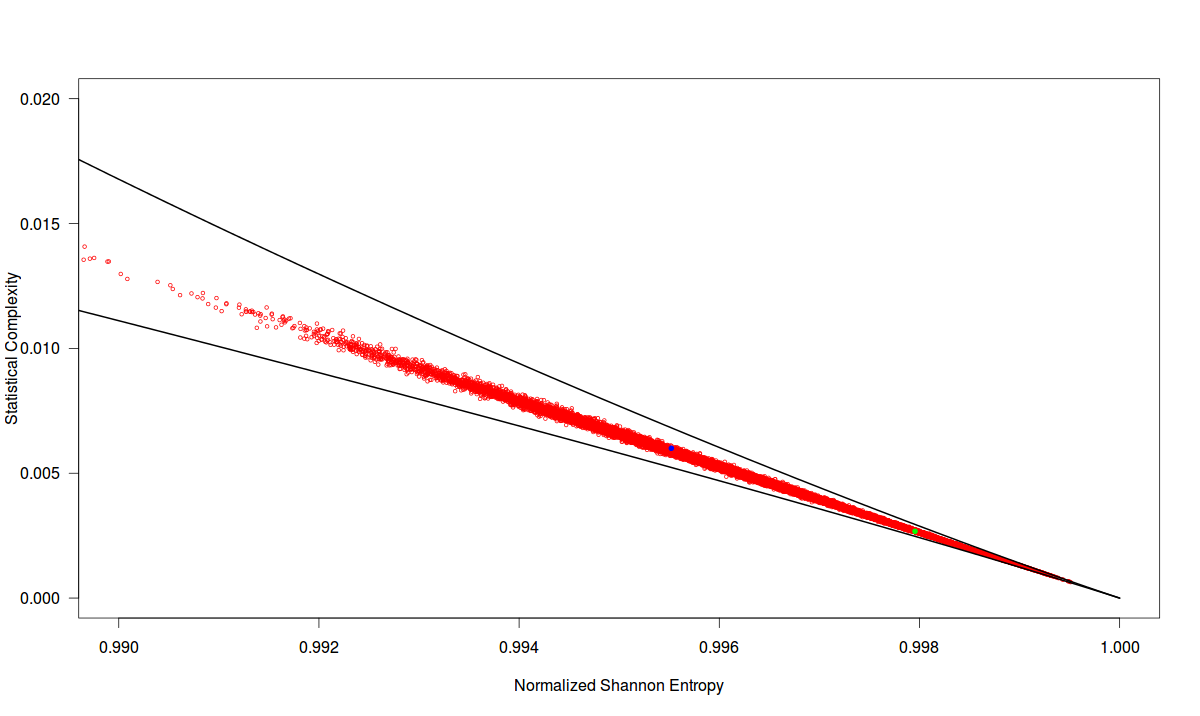
\includegraphics[scale=0.25,center]{../Rplot}
      \caption{$10^3$ pontos no Plano HC}
      \end{figure}
\end{frame}

\begin{frame}{Resultados}
    \begin{block}{P-valor}
    \begin{itemize}
      \item p-valor LCG: $0.135$
      \pause
      \item p-valor MT: $0.850$
      \pause
      \end{itemize}
  \end{block}
    \begin{figure}
      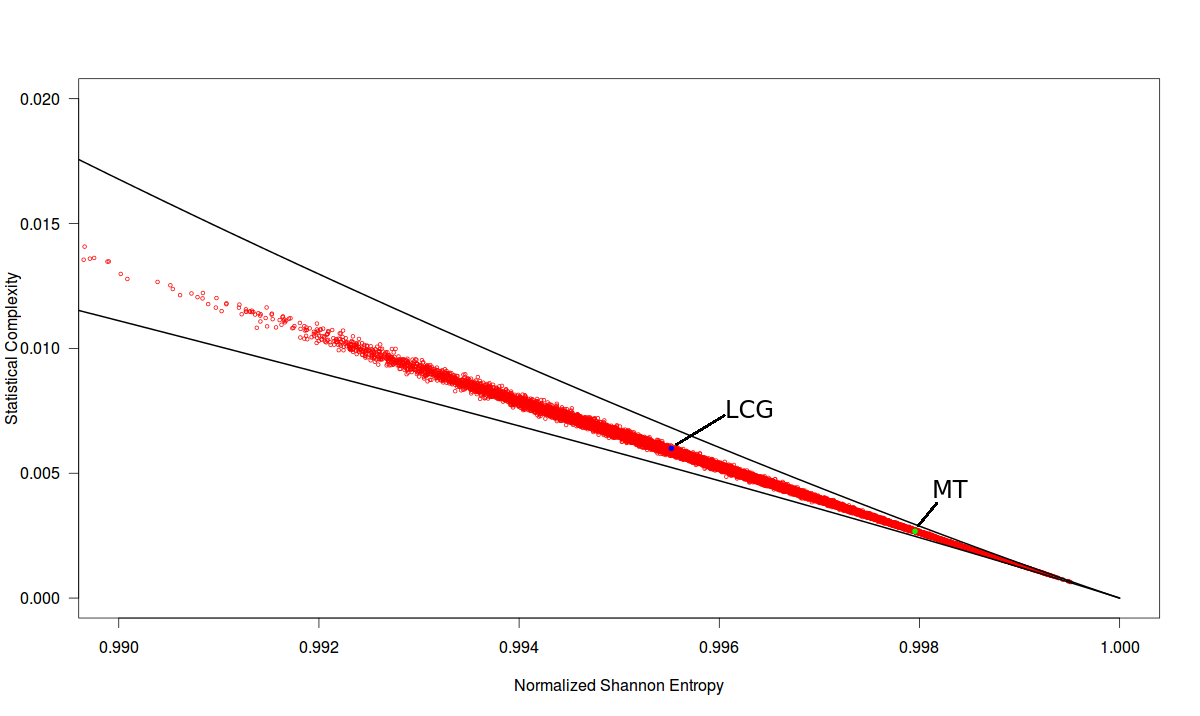
\includegraphics[scale=0.25,center]{../Planck_no_PCA_labels}
      \caption{Pontos LCG e MT}
      \end{figure}
\end{frame}

\begin{frame}{}
    \begin{figure}
      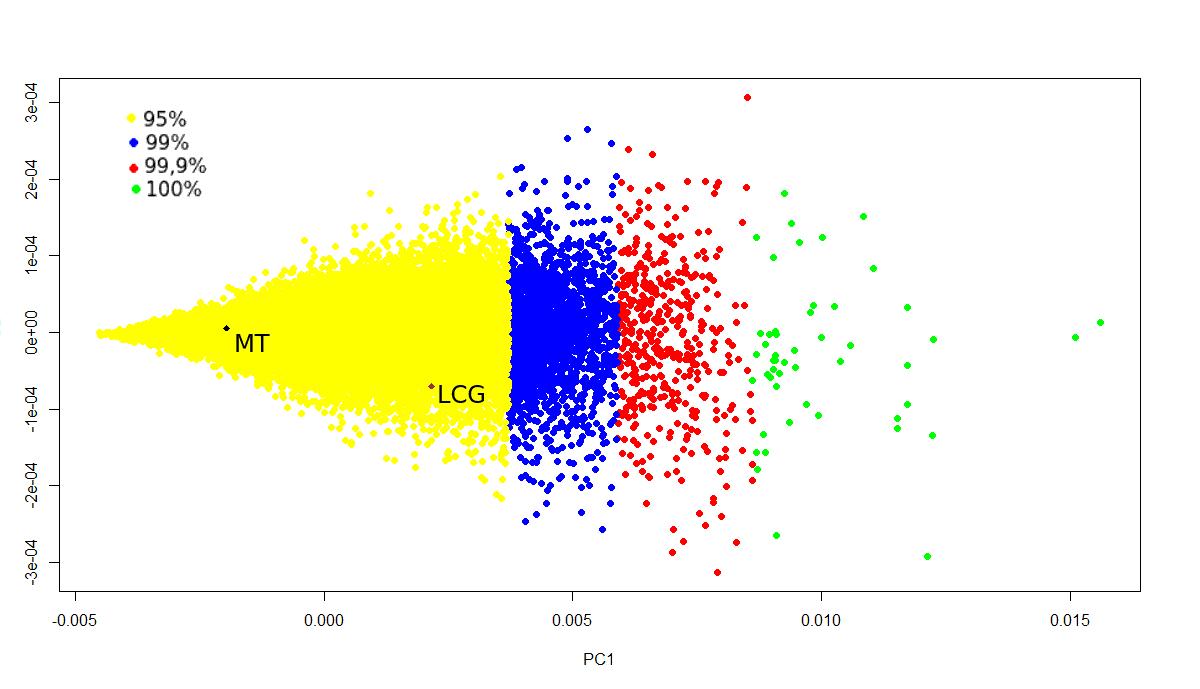
\includegraphics[scale=0.25,center]{../Planck_MT_LCG_labels}
      \caption{Dados submetidos a PCA}
      \end{figure}
\end{frame}


\begin{frame}{Obrigado!}
    \begin{figure}
      
\includegraphics[scale=0.5,center]{thankyou}
      \end{figure}
\end{frame}

\section*{Referências}
\bibliographystyle{../sbc}
\bibliography{../references}

\end{document}